\begin{figure}[H]
\centering
\begin{tcolorbox}[colback=white, colframe=black, boxrule=0.4pt, arc=2pt, left=2mm, right=2mm, top=1mm, bottom=1mm]
\begin{center}
\resizebox{0.8\textwidth}{!}{
  \begin{tikzpicture}[
    every node/.style={draw, minimum width=2.5cm, minimum height=1cm, font=\sffamily},
    level distance=1.8cm,
    sibling distance=3.5cm,
    ->, >=stealth
  ]

  % Nodos
  \node (state1) {$\mathrm{STATE}_{1}$}
    child {node (county1) {$\mathrm{COUNTY}_{1}$} 
      child {node (station1) {$\mathrm{STATION}_{1}$}
        child {node (time1) {$\mathrm{TIME}_{1}$}}
      }
      child {node (stationk) {$\mathrm{STATION}_{j}$}
        child {node (timet) {$\mathrm{TIME}_{t}$}}
      }
    }
    child {node (countyc) {$\mathrm{COUNTY}_{c}$}};

  \node[right=8cm of state1] (statez) {$\mathrm{STATE}_{s}$}
    child {node (others) {$\mathrm{IDENTICAL\ REPRESENTATION}$}};

  \draw[dashed] (county1) -- (countyc);
  \draw[dashed] (station1) -- (stationk);
  \draw[dashed] (time1) -- (timet);
  \draw[dashed] (state1) -- (statez);

  \end{tikzpicture}
}
\end{center}
\end{tcolorbox}
\caption{Hierarchical structure of the multilevel model: states, counties, stations, and time.}
\label{fig:hierarchy}
\end{figure}


\begin{figure}[h]
    \centering
    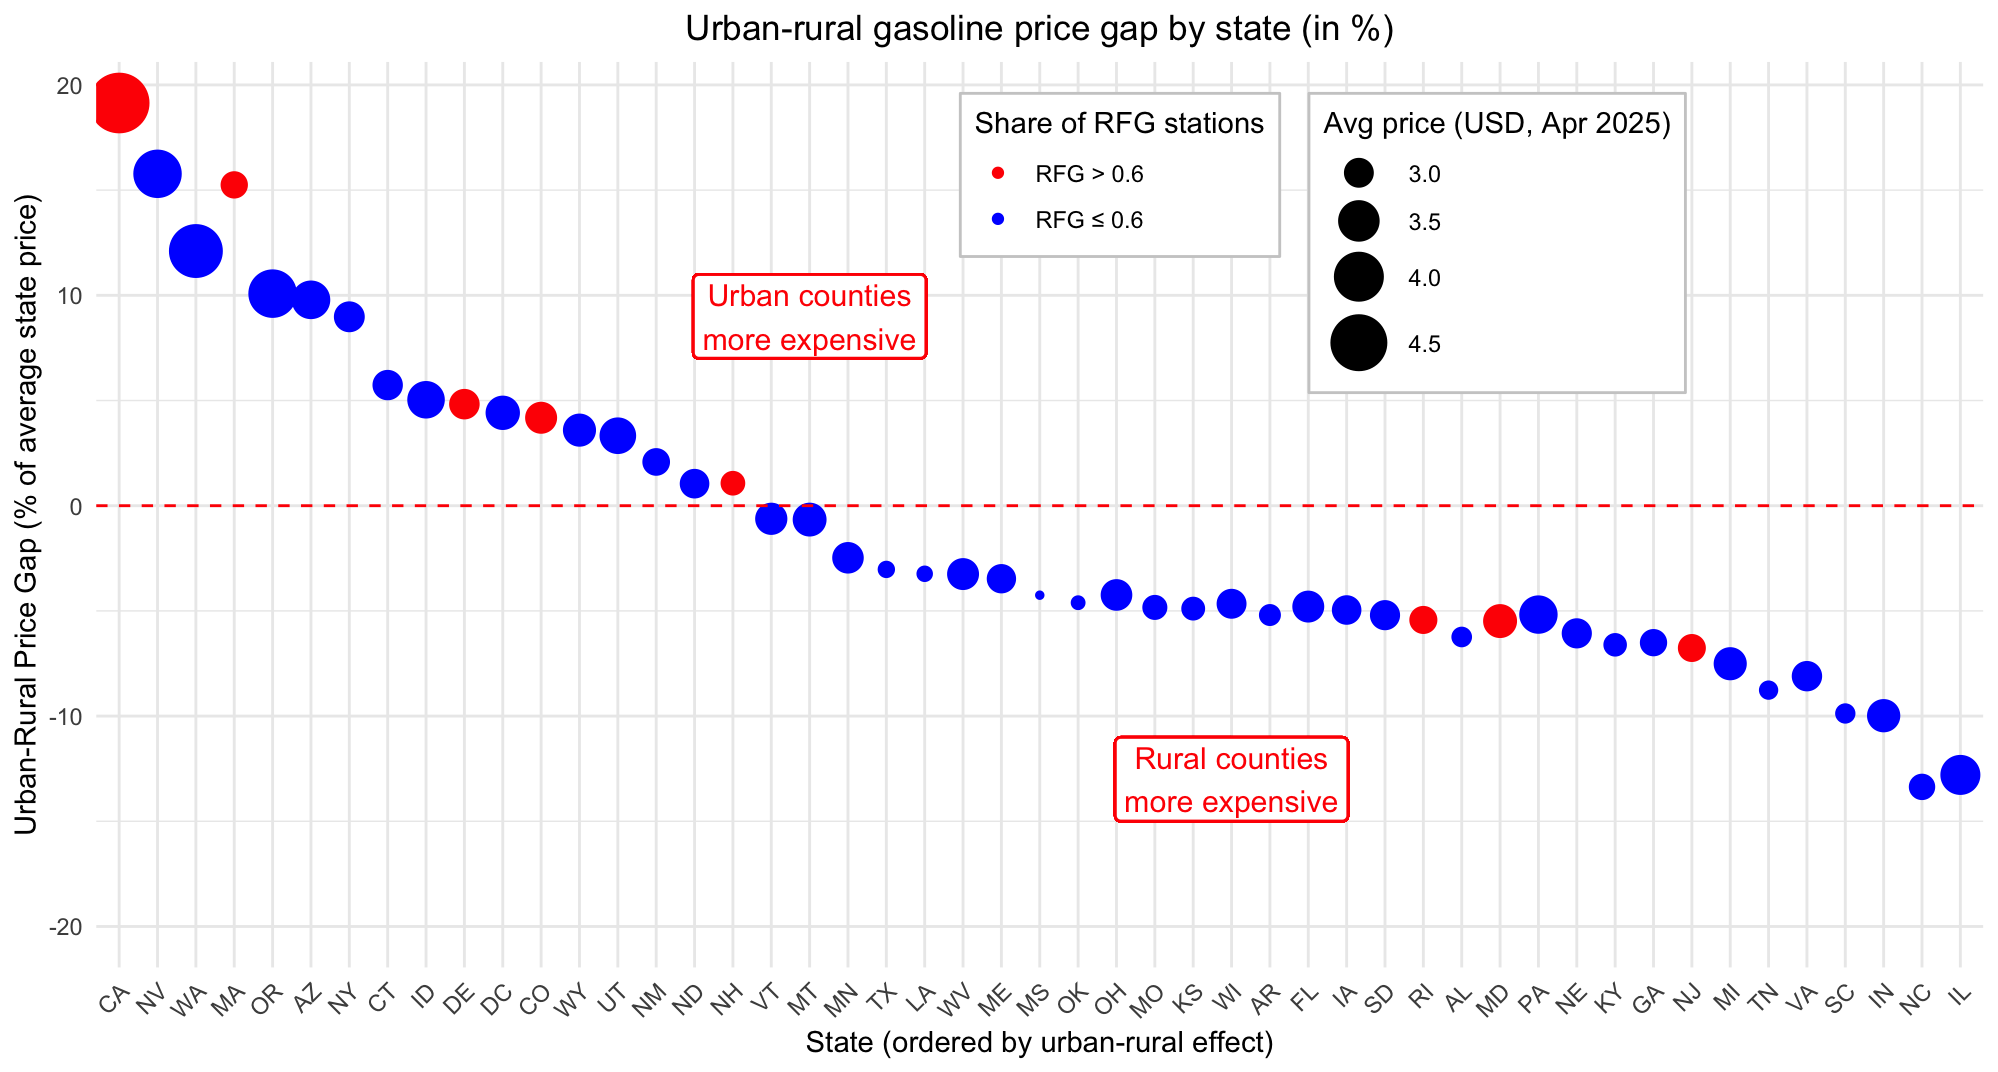
\includegraphics[width=\linewidth]{Figures/Rplot02.png}
\caption{State-Level Urban–Rural Gasoline Price Gaps (as Percentage of State Average)}

    \label{fig:Figure2}
\end{figure}

\newpage